\begin{tikzpicture}
\shorthandoff{>}
%
\pgfmathdeclarefunction{sha}{1}{\pgfmathparse{#1*log2(#1)}};
%
% Concavidad de - u log u
\begin{scope}[xscale=4,yscale=3.5]
\pgfmathsetmacro{\u}{.125};
\pgfmathsetmacro{\v}{.85};
\pgfmathsetmacro{\l}{.7};
\pgfmathsetmacro{\cc}{\l*\u+(1-\l)*\v};
%
% Axis
\draw[>=stealth,->] (-.1,0)--(1.3,0) node[right,scale=.8]{$t$};
\draw[>=stealth,->] (0,{1.05*sha(2^(-1/ln(2)))})--(0,{sha(1.25)})
node[above,scale=.8]{$\phi(t) = t \log t$};
%
\node[below left,scale=.8] at (0,0){$0$};
\draw (1,0)--(1,-.05) node[below,scale=.8]{$1$};

\draw[thick,domain=.005:1,samples=200] (0,0)-- plot (\x,{sha(\x)});
\draw[dotted,domain=1:1.25,samples=200] (0,0)-- plot (\x,{sha(\x)});
\draw[dashed] (\u,{sha(\u)})--(\v,{sha(\v)});
%
\draw[dotted] (\u,0)--(\u,{sha(\u)}) node[scale=.6]{$\bullet$} node[below,scale=.8]{$A_1$} ;
\draw (\u,0)--(\u,-.025) node[below,scale=.8]{$t_1$};
%
\draw[dotted] (\v,0)--(\v,{sha(\v)}) node[scale=.6]{$\bullet$} node[below,scale=.8]{$A_2$} ;
\draw (\v,0)--(\v,-.025) node[below,scale=.8]{$t_2$};
%
\draw[dashed] (\cc,.025) node[above,scale=.8]{$\pi_1 t_1 + \pi_2 t_2$}
--(\cc,{sha(\cc)}) node[scale=.6]{$\bullet$} node[below,scale=.8]{$A_\pi$};
%
% l phi(u) + (1-l) phi(v)
\draw[dotted]
(\cc,{\l*sha(\u)+(1-\l)*sha(\v)})--(0,{\l*sha(\u)+(1-\l)*sha(\v)});
%node[left,scale=.8]{$\pi_1 \phi(t_1) + \pi_2 \phi(t_2)$};
\draw
(0,{\l*sha(\u)+(1-\l)*sha(\v)})--(-.025,{\l*sha(\u)+(1-\l)*sha(\v)})
node[left,scale=.8]{$\pi_1 \phi(t_1) + \pi_2 \phi(t_2)$};
%
\node[scale=.6] at ({\l*\u+(1-\l)*\v},{\l*sha(\u)+(1-\l)*sha(\v)}){$\bullet$};
%
% phi(l u + (1-l) v)
\draw[dotted] (\cc,{sha(\cc)})--(0,{sha(\cc)});
\draw (0,{sha(\cc)})--(-.025,{sha(\cc)})
node[left,scale=.8]{$\phi(\pi_1 t_1 + \pi_2 t_2)$};
\end{scope}
%
%
% Concavidad / mezcla
\begin{scope}[xshift=8.5cm]
\draw(0,1) node{\includegraphics[width=3cm]{TIKZ_SZ/DosDados}};
\node[scale=.8] at (-.5,2.25){$p_{(1)}$};
\node[scale=.8] at (1,1.75){$p_{(2)}$};
\node[scale=.8] at (2.7,.75){$\pi_1 p_{(1)} + \pi_2 p_{(2)}$};
\node at (-.25,-1.5){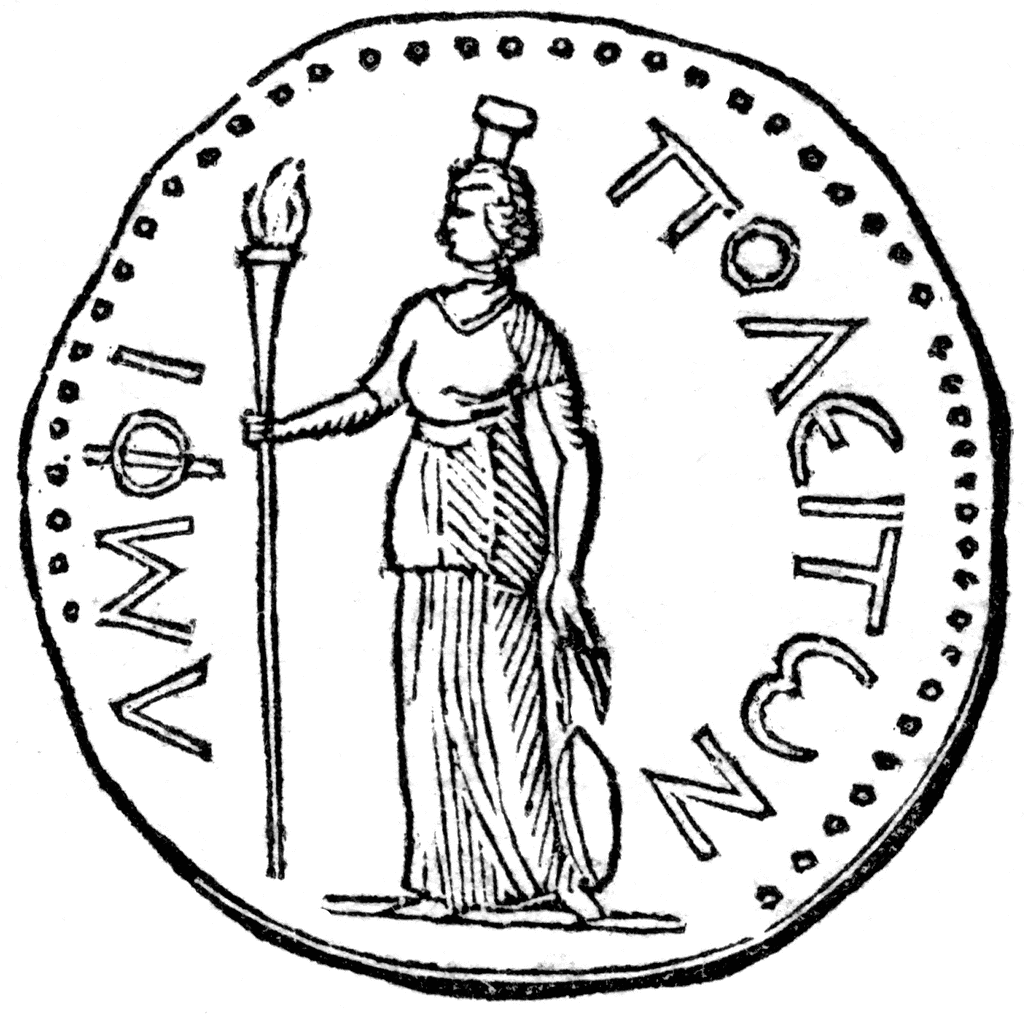
\includegraphics[width=1cm]{TIKZ_SZ/Moneda}};
\draw[>=stealth,->,thick] (-.3,-.75)--(-.75,.15);
\node[left,scale=.8] at (-.525,-.35){$\pi_1$};
\draw[>=stealth,->,thick] (-.2,-.75)--(.3,.15);
\node[right,scale=.8] at (.05,-.35){$\pi_2 = 1-\pi_1$};
\end{scope}
%
\node at (1.25,-2.75){(a)};
\node at (8.25,-2.75){(b)};
\end{tikzpicture}
